\documentclass[a4paper,12pt]{article}

\usepackage[utf8]{inputenc}
\usepackage[T1]{fontenc}
\usepackage[italian]{babel}
\usepackage{enumitem}
\usepackage{geometry}
\usepackage{hyperref}
\usepackage{booktabs}
\usepackage{graphicx}
\usepackage{longtable}

\geometry{margin=2.5cm}

\title{Documentazione Tecnica di Progetto \\ \large Gestionale Locale per la Gestione del Magazzino}
\author{Gruppo 11}
\date{26 Maggio 2026}

\begin{document}

\maketitle

\section*{Storico delle Versioni}
\begin{center}
    \begin{tabular}{llll}
        \toprule
        \textbf{Versione} & \textbf{Data} & \textbf{Descrizione}                                          & \textbf{Autore} \\
        \midrule
        v1.0              & 26/05/2026    & Strutturazione iniziale, analisi requisiti e allineamento UML & Gruppo 11       \\
        \bottomrule
    \end{tabular}
\end{center}

\newpage
\tableofcontents
\newpage

\section{Introduzione}
\subsection{Scopo del Progetto}
Il software ha l'obiettivo di gestire le dinamiche logistiche interne di un'azienda, ottimizzando la gestione del magazzino, della movimentazione delle merci in entrata/uscita e della documentazione contabile associata.

\subsection{Obiettivi e Ambito (Scope)}
L'applicazione opera in un contesto puramente locale (offline). Questa scelta risponde a specifici vincoli ambientali e di sicurezza dell'infrastruttura ospitante, la quale potrebbe presentare zone prive di connettività internet stabile o politiche aziendali restrittive riguardo all'esposizione di dati sensibili all'esterno della rete aziendale. Il sistema gestisce l'intero ciclo di vita della merce: dalla registrazione dei prodotti a magazzino alla generazione dei documenti di trasporto (DDT) e della fatturazione.

\subsection{Glossario}
\begin{itemize}
    \item \textbf{DDT}: Documento di Trasporto.
    \item \textbf{RBAC}: Role-Based Access Control (Gestione permessi basata sui ruoli).
    \item \textbf{MVC}: Model-View-Controller (Pattern architetturale).
    \item \textbf{DAO}: Data Access Object (Oggetto per l'accesso ai dati).
    \item \textbf{Stock-out}: Condizione di esaurimento delle scorte di un prodotto.
\end{itemize}

\section{Analisi dei Requisiti}
\subsection{Attori del Sistema}
\begin{itemize}
    \item \textbf{Magazziniere}: Gestisce il flusso fisico delle merci (carico/scarico), effettua la scansione dei codici a barre, consulta le giacenze e genera i DDT per la merce in uscita.
    \item \textbf{Contabile}: Visiona l'elenco e il dettaglio degli ordini, gestisce le fatture, le note di credito e modifica i listini dei prezzi di acquisto e vendita.
    \item \textbf{Amministratore}: Supervisione globale del sistema, consultazione delle merci e dei prezzi, controllo delle fatture, gestione dei resi e generazione della reportistica avanzata dell'inventario.
\end{itemize}

\subsection{Requisiti Funzionali (RF)}
\begin{longtable}{p{0.15\textwidth} p{0.6\textwidth} p{0.15\textwidth}}
    \caption{Requisiti Funzionali}                                                                                                              \\
    \toprule
    \textbf{ID} & \textbf{Descrizione}                                                                                      & \textbf{Priorità} \\
    \midrule
    RF-01       & Login degli utenti tramite username e password basato su ruoli (RBAC).                                    & Alta              \\
    RF-02       & Blocco automatico dell'account utente a seguito di 3 tentativi di login falliti.                          & Alta              \\
    RF-03       & Recupero della password utente tramite verifica di una domanda di sicurezza preimpostata.                 & Media             \\
    RF-04       & Visualizzazione, inserimento e modifica dei dati anagrafici dei prodotti e delle categorie.               & Alta              \\
    RF-05       & Consultazione in tempo reale dell'elenco delle giacenze di magazzino.                                     & Alta              \\
    RF-06       & Registrazione di un nuovo Ordine di Entrata e aggiornamento automatico incrementale delle giacenze.       & Alta              \\
    RF-07       & Registrazione di un nuovo Ordine di Uscita e decremento automatico delle giacenze dei prodotti coinvolti. & Alta              \\
    RF-08       & Generazione automatica di un DDT per ogni Ordine di Uscita evaso.                                         & Alta              \\
    RF-09       & Passaggio automatico dello stato dell'Ordine di Uscita da "Confermato" a "Evaso" alla creazione del DDT.  & Alta              \\
    RF-10       & Notifica visiva immediata per i prodotti la cui giacenza scende sotto la soglia minima di sicurezza.      & Media             \\
    RF-11       & Consultazione e gestione dei resi della merce con relativo ripristino delle quantità in giacenza.         & Media             \\
    RF-12       & Visualizzazione e filtraggio degli ordini ricevuti (evasi e non evasi) da parte del contabile.            & Alta              \\
    RF-13       & Generazione e conservazione di fatture di vendita e note di credito con numerazione progressiva annuale.  & Alta              \\
    RF-14       & Modifica manuale dei listini dei prezzi di vendita e di acquisto dei prodotti.                            & Media             \\
    RF-15       & Integrazione software per l'acquisizione rapida dei codici a barre dei prodotti tramite lettore ottico.   & Media             \\
    \bottomrule
\end{longtable}

\subsection{Requisiti Non Funzionali (RNF)}
\begin{longtable}{p{0.15\textwidth} p{0.25\textwidth} p{0.45\textwidth}}
    \caption{Requisiti Non Funzionali}                                                                                                                     \\
    \toprule
    \textbf{ID} & \textbf{Categoria} & \textbf{Descrizione}                                                                                                \\
    \midrule
    RNF-01      & Prestazioni        & Il tempo di risposta alla scansione di un codice a barre deve essere inferiore a 0.5s per il 95\% delle operazioni. \\
    RNF-02      & Prestazioni        & La generazione di un report annuale dell'inventario non deve richiedere più di 3s di elaborazione CPU.              \\
    RNF-03      & Portabilità        & Funzionamento garantito in modalità offline su qualsiasi sistema operativo desktop moderno.                         \\
    RNF-04      & Sicurezza          & Dati archiviati interamente in locale senza alcuna esposizione o transito all'esterno della rete aziendale.         \\
    RNF-05      & Archiviazione      & Utilizzo di un database embedded SQLite, memorizzato in un singolo file binario locale.                             \\
    RNF-06      & Usabilità          & Interfaccia grafica (GUI) leggera, reattiva e ottimizzata per hardware a risorse limitate.                          \\
    \bottomrule
\end{longtable}

\subsection{Analisi dei Casi d'Uso}
Il sistema è documentato tramite diagrammi dei casi d'uso che mappano le interazioni tra i tre attori principali e le macro-funzionalità del sistema. I flussi dettagliati delle operazioni principali sono descritti nei diagrammi di attività allegati nella cartella di progetto.

\begin{figure}[h]
    \centering
    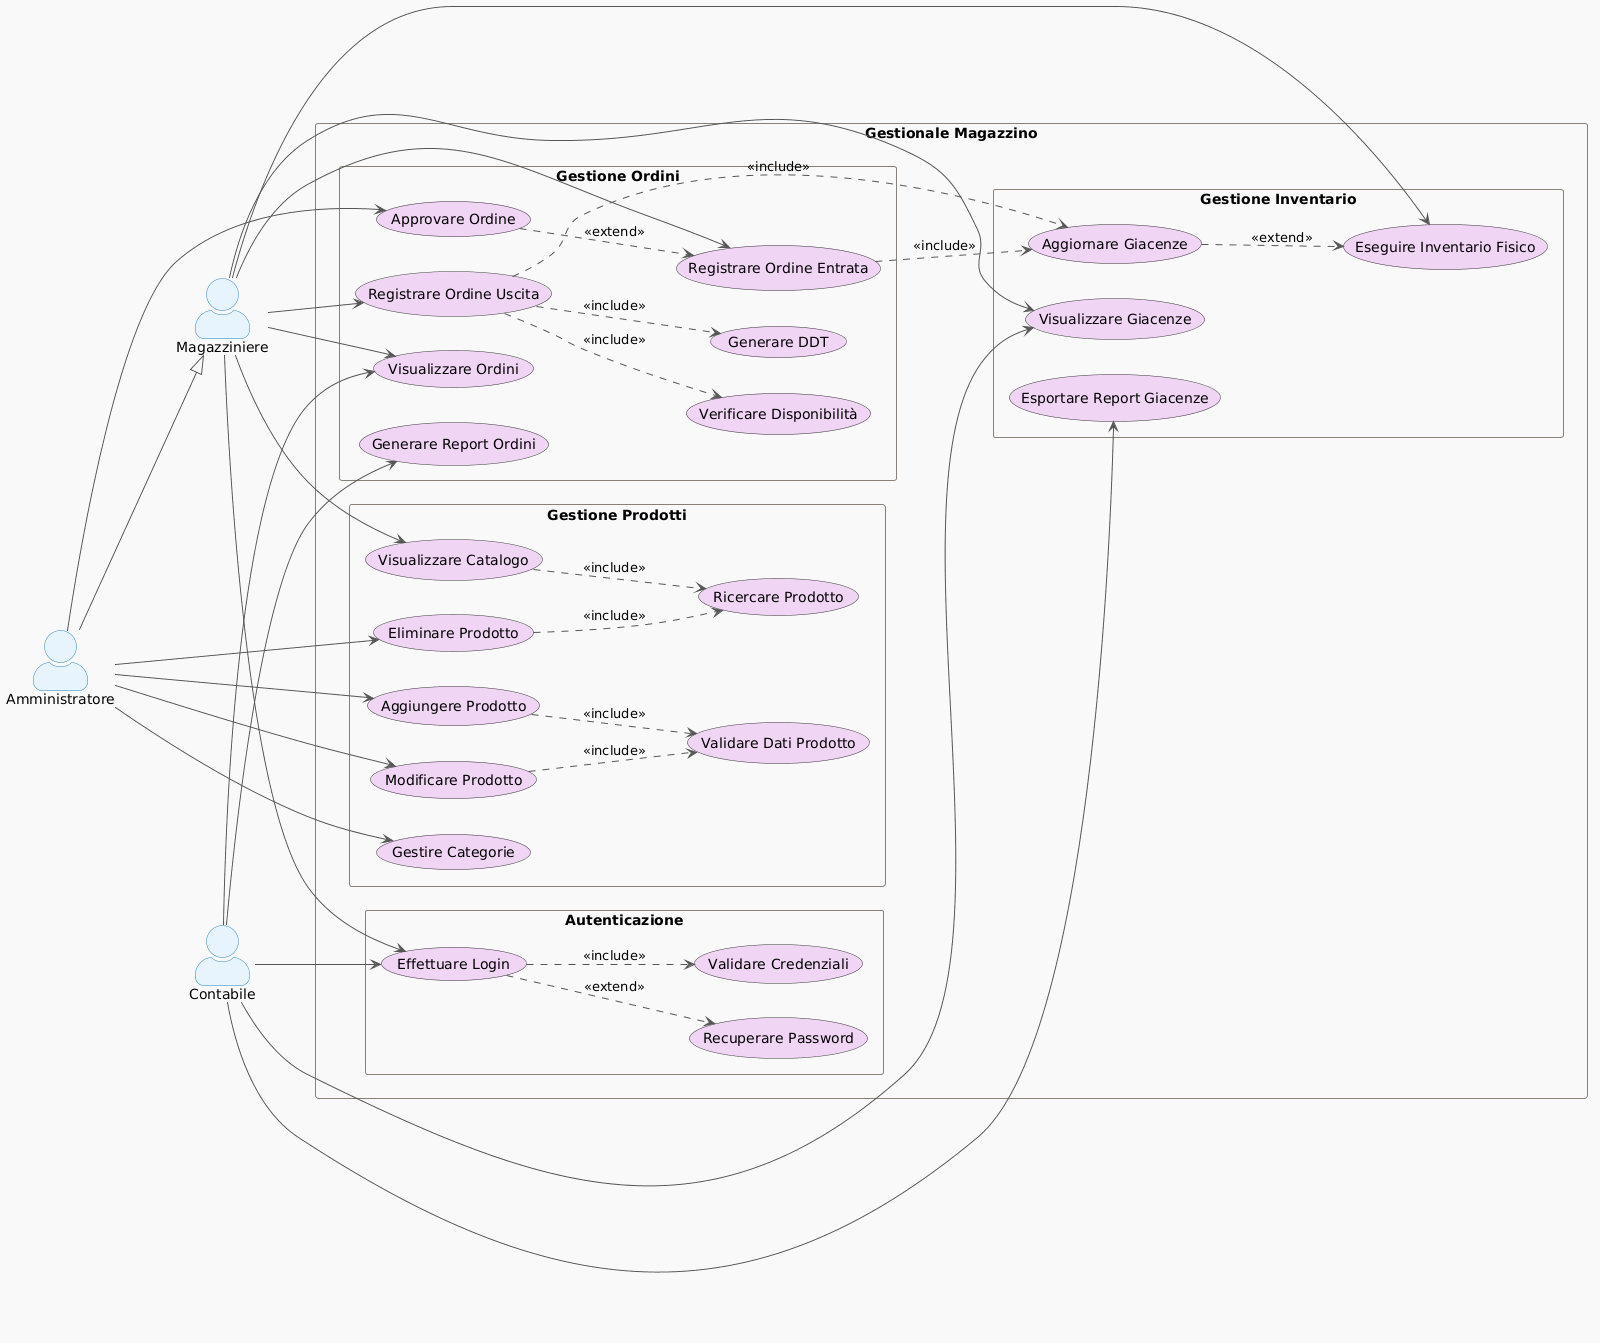
\includegraphics[width=0.8\textwidth]{./img/png-uml/UseCaseDiagram.png}
    \caption{Diagramma dei Casi d'Uso Generale}
\end{figure}

\section{Progettazione e Architettura}
\subsection{Scelte Architetturali}
Il software adotta rigorosamente il pattern architetturale \textbf{Model-View-Controller (MVC)}. Questa scelta garantisce la netta separazione tra la logica di business e l'interfaccia utente, abbattendo il debito tecnico. Il motore di database scelto è \textbf{SQLite} per rispondere al vincolo di esecuzione locale e portabilità assoluta (zero configurazione iniziale, assenza di demoni di rete in background e facilità di backup tramite la copia di un singolo file binario).

\subsection{Modello del Dominio}
Il dominio dell'applicazione è incentrato sulle entità fondamentali per il tracciamento logistico, mappate nel file \texttt{Domain\_model.puml}: \texttt{Utente}, \texttt{Prodotto}, \texttt{Categoria}, \texttt{Giacenza}, \texttt{OrdineEntrata}, \texttt{OrdineUscita} e \texttt{DDT}.

\begin{figure}[h]
    \centering
    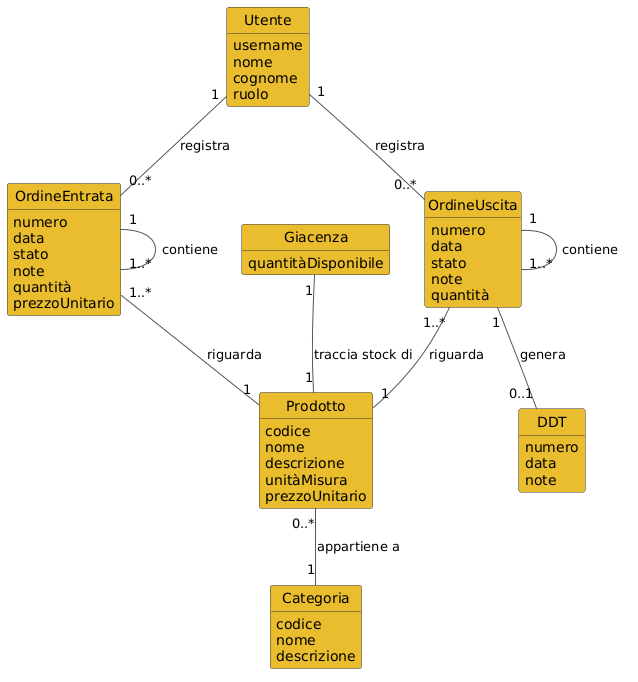
\includegraphics[width=0.8\textwidth]{./img/png-uml/DomainModel.png}
    \caption{Modello del Dominio}
\end{figure}

\subsection{Design Dettagliato (Diagramma delle Classi)}
La struttura interna del codice segue rigorosamente lo schema delle classi definito in \texttt{Class\_diagram.puml}. Per isolare la persistenza dei dati, viene adottato il pattern \textbf{DAO (Data Access Object)}. Le classi DAO incapsulano la totalità delle istruzioni SQL ed eseguono le query sul database SQLite, garantendo che lo strato dei Controller dipenda esclusivamente da oggetti di dominio e mai dal dialetto SQL sottostante.

\begin{figure}[h]
    \centering
    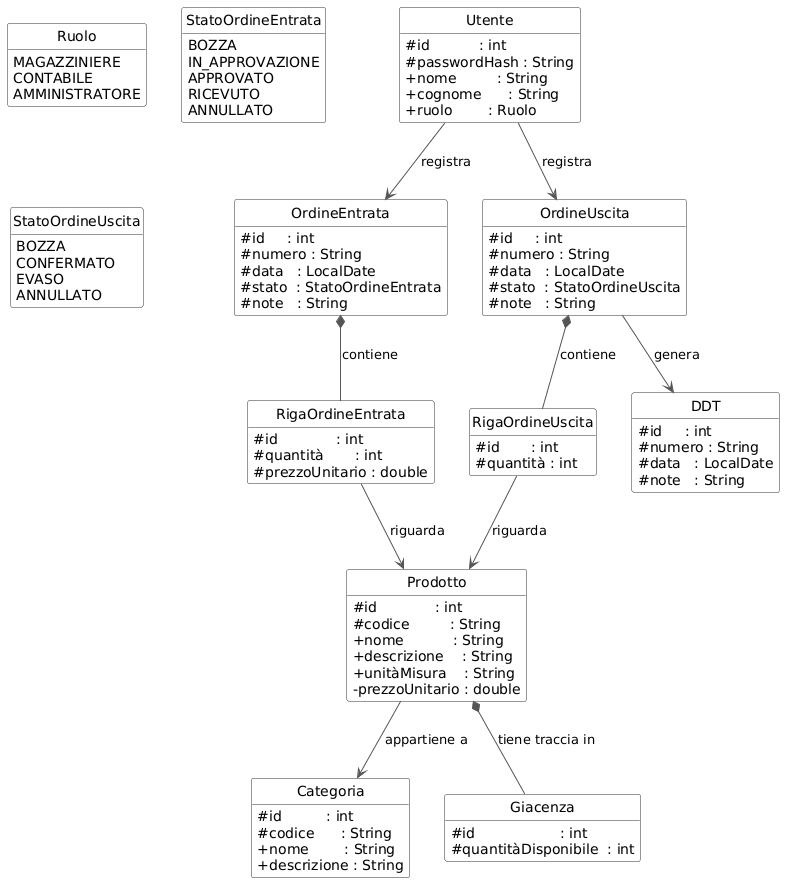
\includegraphics[width=0.9\textwidth]{./img/png-uml/ClassDiagram.png}
    \caption{Diagramma delle Classi}
\end{figure}

\subsection{Comportamento del Sistema (Diagrammi di Sequenza)}
I flussi di interazione dinamica tra i componenti della View, della logica di controllo (Service) e dello strato dei dati sono formalizzati tramite diagrammi di sequenza. Di seguito viene riportato, a titolo esemplificativo, il diagramma di sequenza relativo al processo di login e recupero delle credenziali (\texttt{UC1\_login\_sequence.puml}).

\begin{figure}[h]
    \centering
    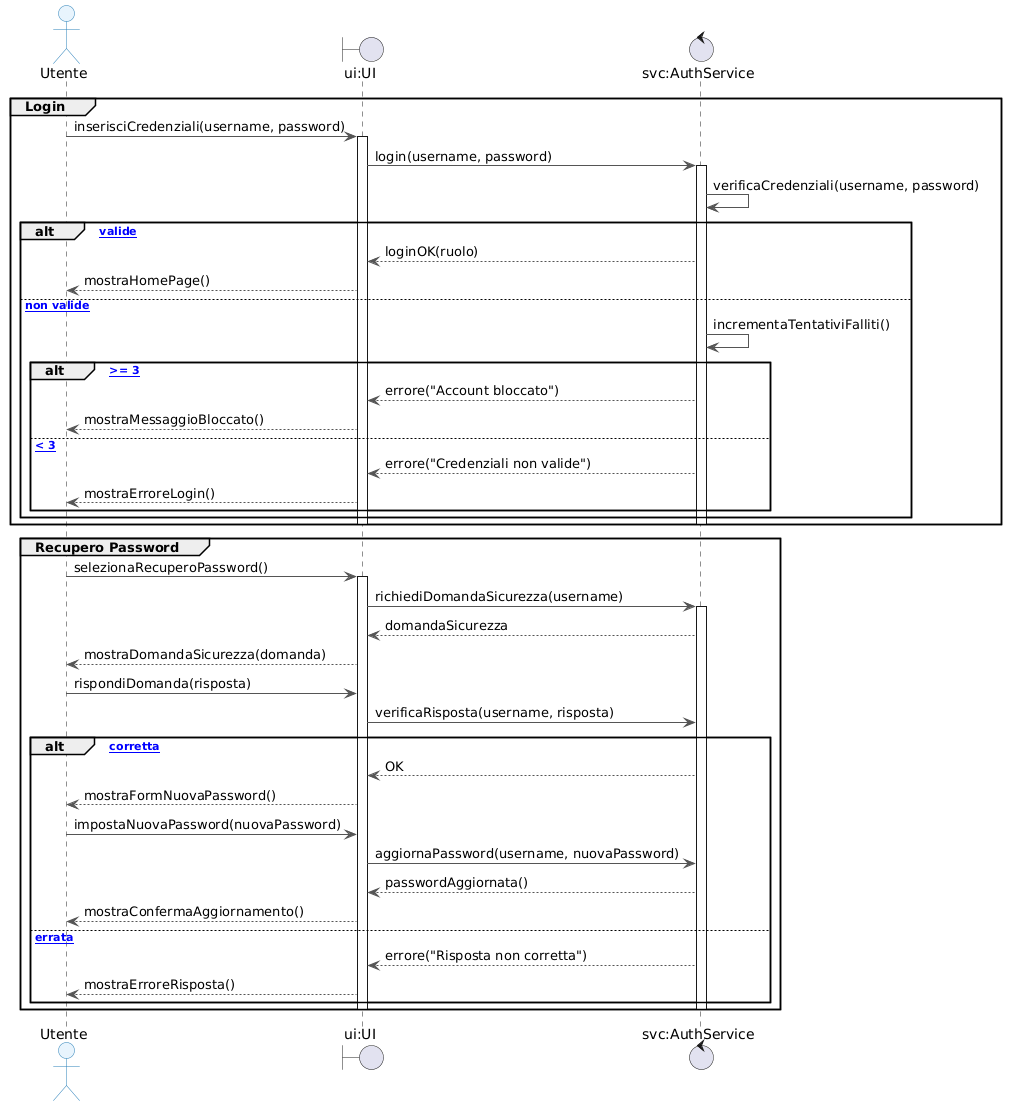
\includegraphics[width=0.8\textwidth]{./img/png-uml/UC1_Login_SD.png}
    \caption{Diagramma di Sequenza: Login e Recupero Password (UC1)}
\end{figure}

\begin{figure}[h]
    \centering
    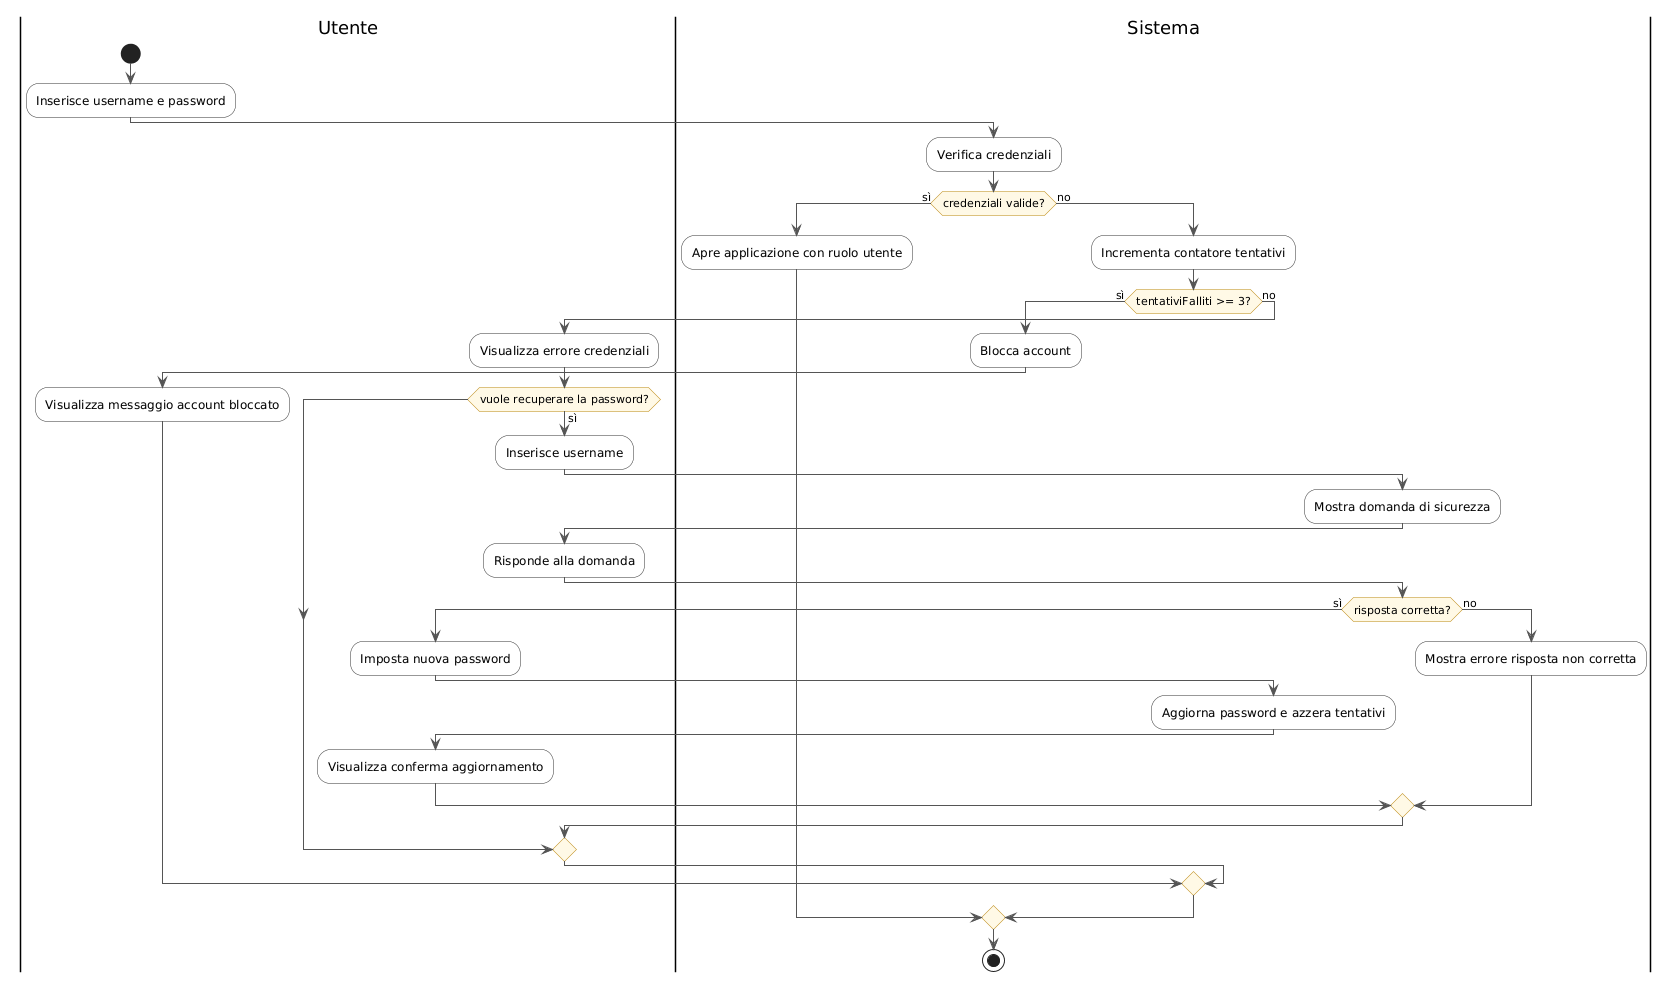
\includegraphics[width=0.8\textwidth]{./img/png-uml/UC1_Login_AD.png}
    \caption{Diagramma di Attività: Login e Recupero Password (UC1)}
\end{figure}

\begin{figure}[h]
    \centering
    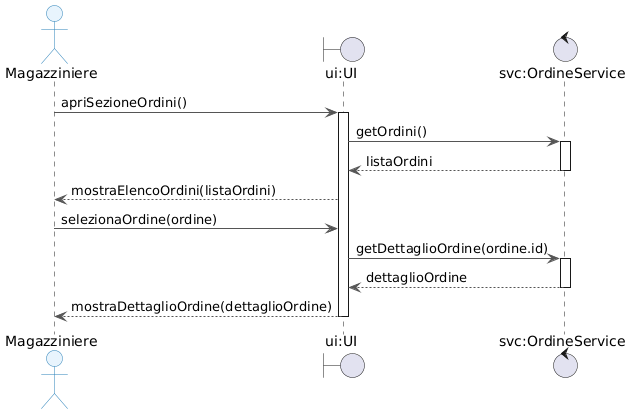
\includegraphics[width=0.8\textwidth]{./img/png-uml/UC2_VisualizzaOrdini_SD.png}
    \caption{Diagramma di Sequenza: Visualizzazione Ordini (UC2)}
\end{figure}

\begin{figure}[h]
    \centering
    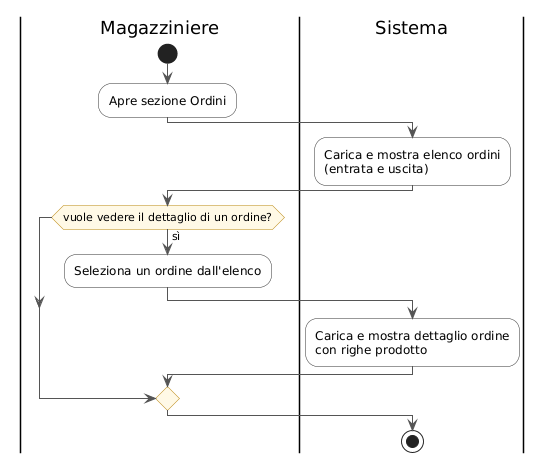
\includegraphics[width=0.8\textwidth]{./img/png-uml/UC2_VisualizzaOrdini_AD.png}
    \caption{Diagramma di Attività: Visualizzazione Ordini (UC2)}
\end{figure}

\begin{figure}[h]
    \centering
    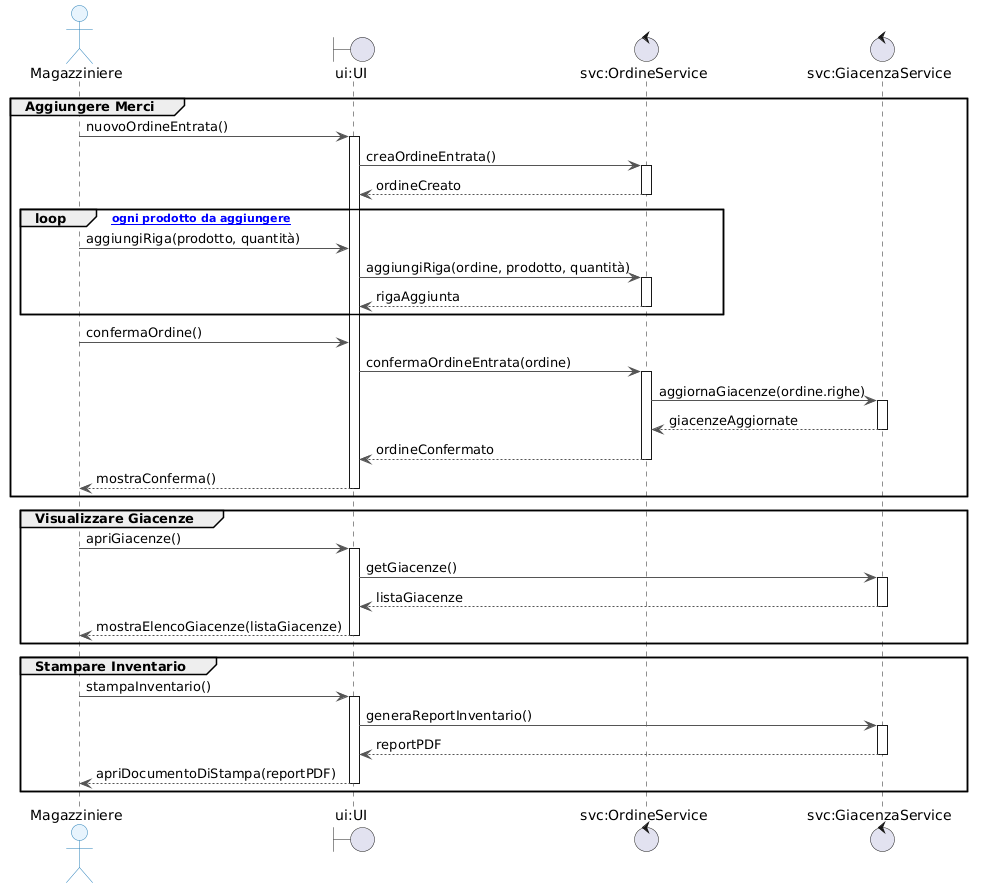
\includegraphics[width=0.8\textwidth]{./img/png-uml/UC3_GestioneGiacenze_SD.png}
    \caption{Diagramma di Sequenza: Gestione Giacenza (UC3)}
\end{figure}

\begin{figure}[h]
    \centering
    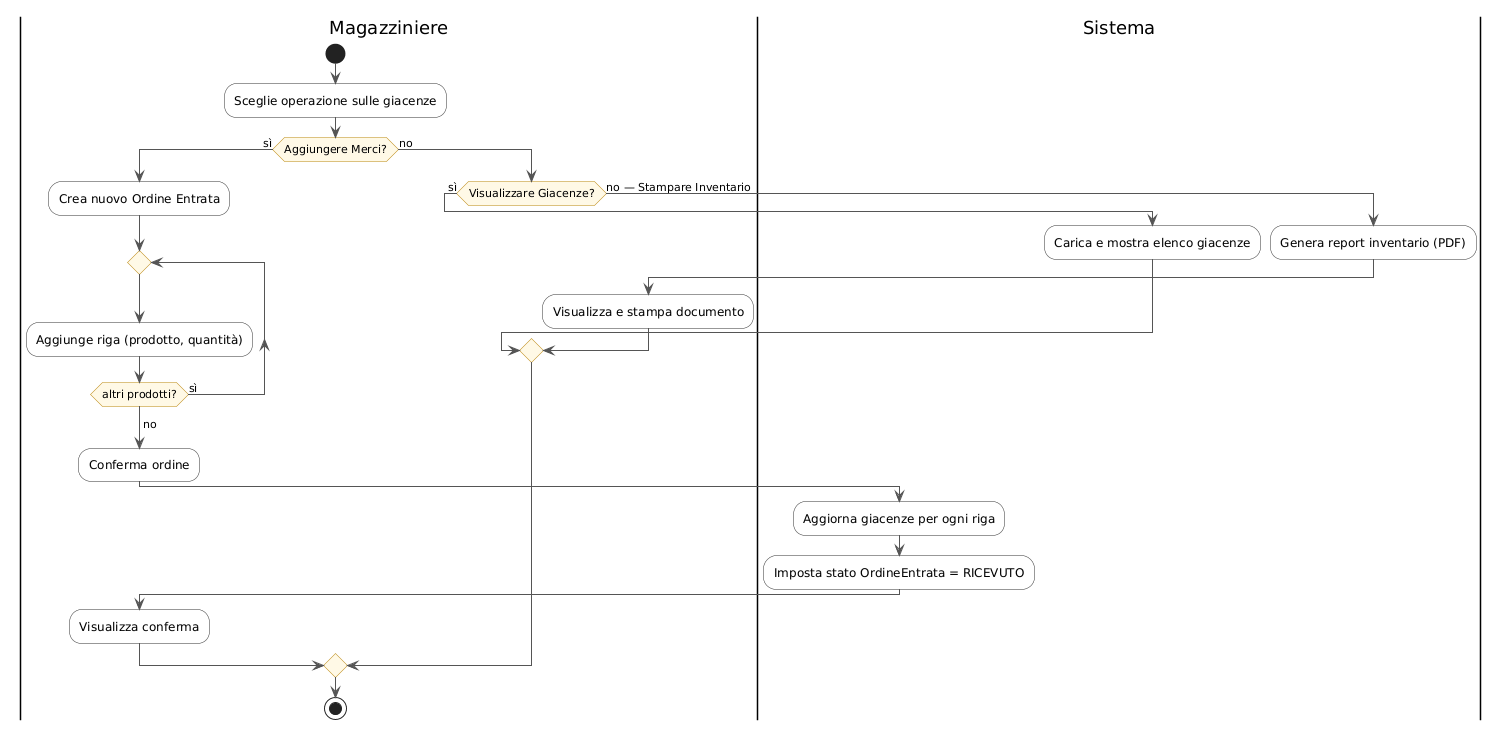
\includegraphics[width=0.8\textwidth]{./img/png-uml/UC3_GestioneGiacenze_AD.png}
    \caption{Diagramma di Attività: Gestione Giacenza (UC3)}
\end{figure}

\begin{figure}[h]
    \centering
    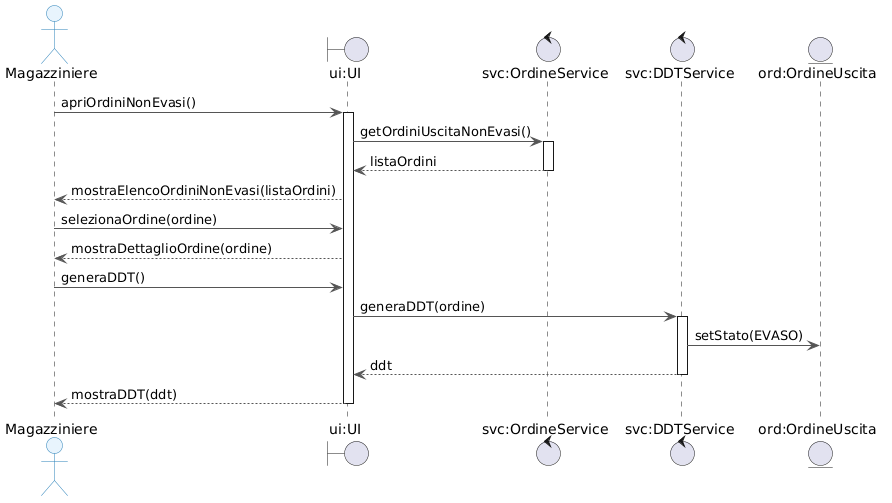
\includegraphics[width=0.8\textwidth]{./img/png-uml/UC4_GeneraDDT_SD.png}
    \caption{Diagramma di Sequenza: Generazione DDT (UC4)}
\end{figure}

\begin{figure}[h]
    \centering
    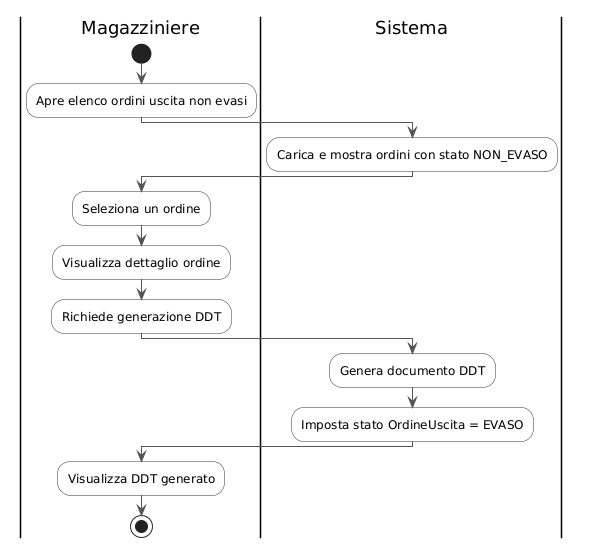
\includegraphics[width=0.8\textwidth]{./img/png-uml/UC4_GeneraDDT_AD.png}
    \caption{Diagramma di Attività: Generazione DDT (UC4)}
\end{figure}

\begin{figure}[h]
    \centering
    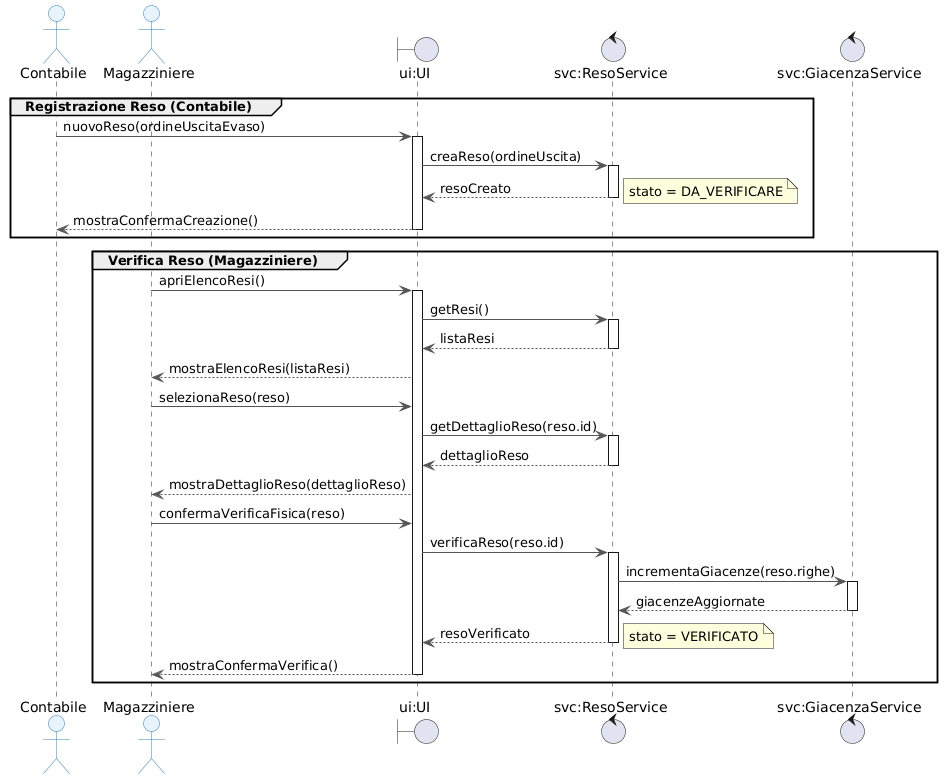
\includegraphics[width=0.8\textwidth]{./img/png-uml/UC5_Resi_SD.png}
    \caption{Diagramma di Sequenza: Resi (UC5)}
\end{figure}

\begin{figure}[h]
    \centering
    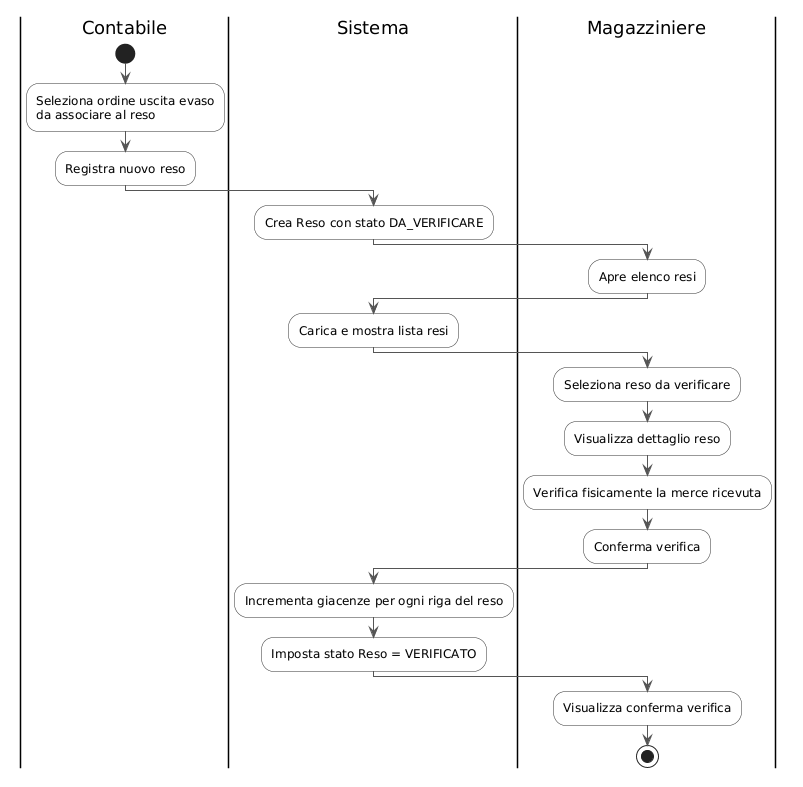
\includegraphics[width=0.8\textwidth]{./img/png-uml/UC5_Resi_AD.png}
    \caption{Diagramma di Attività: Resi (UC5)}
\end{figure}

\begin{figure}[h]
    \centering
    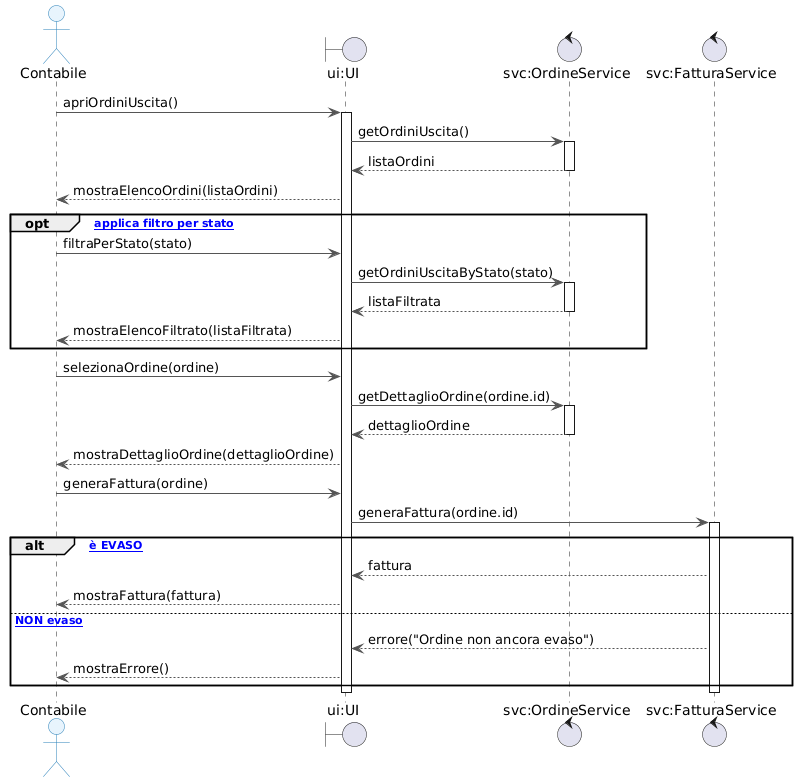
\includegraphics[width=0.8\textwidth]{./img/png-uml/UC6_ContabileOrdini_SD.png}
    \caption{Diagramma di Sequenza: Contabile Ordini (UC6)}
\end{figure}

\begin{figure}[h]
    \centering
    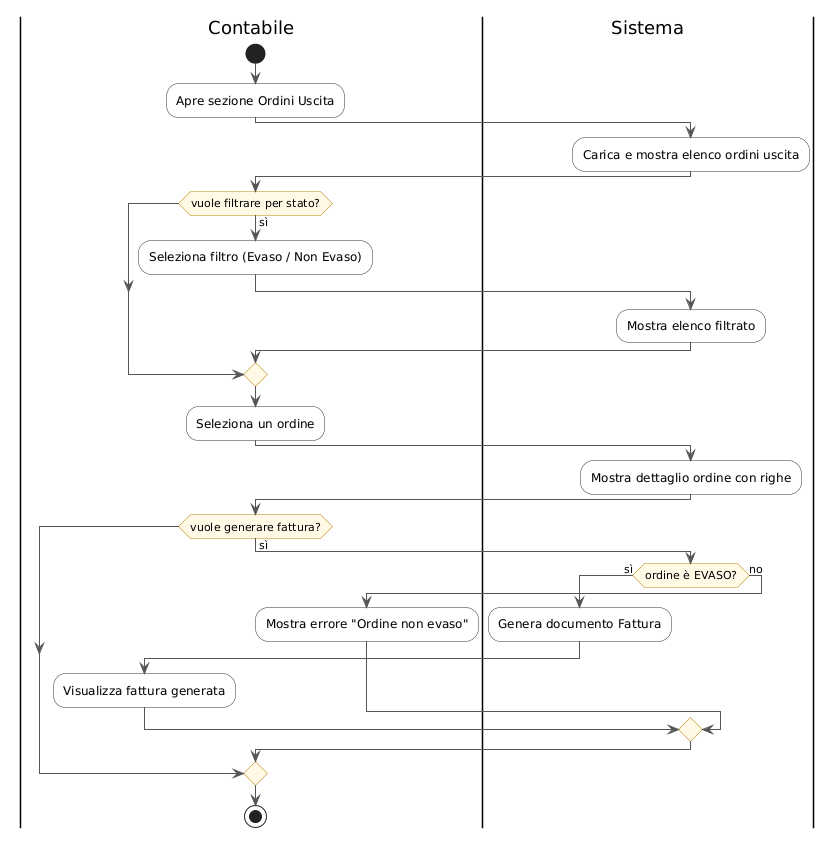
\includegraphics[width=0.8\textwidth]{./img/png-uml/UC6_ContabileOrdini_AD.png}
    \caption{Diagramma di Attività: Contabile Ordini (UC6)}
\end{figure}

\begin{figure}[h]
    \centering
    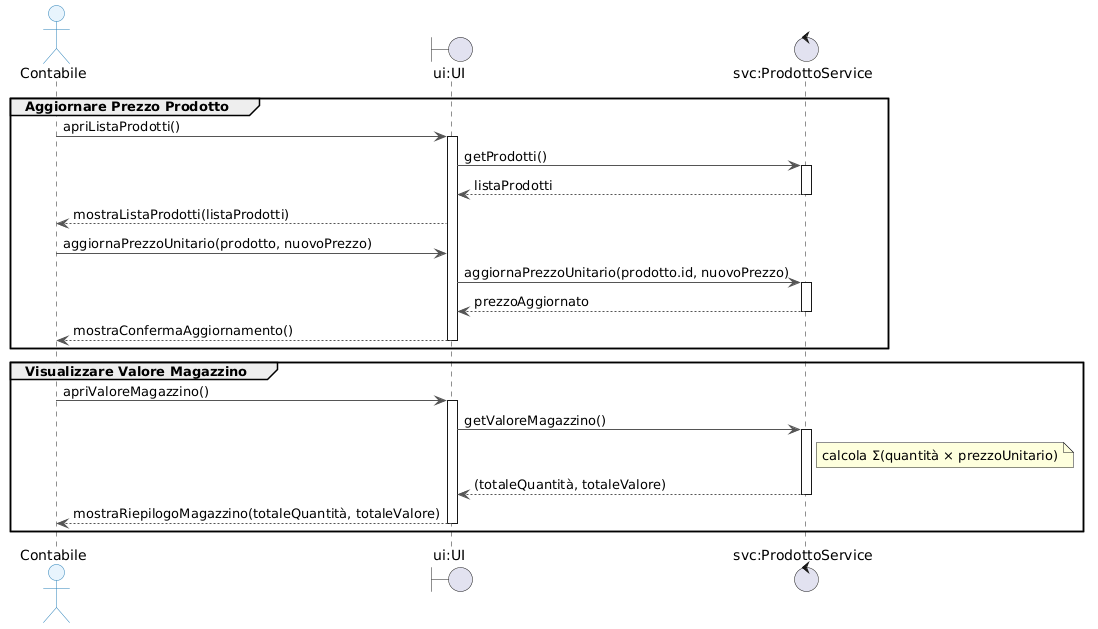
\includegraphics[width=0.8\textwidth]{./img/png-uml/UC7_ContabilePrezzi_SD.png}
    \caption{Diagramma di Sequenza: Contabile Prezzi (UC7)}
\end{figure}

\begin{figure}[h]
    \centering
    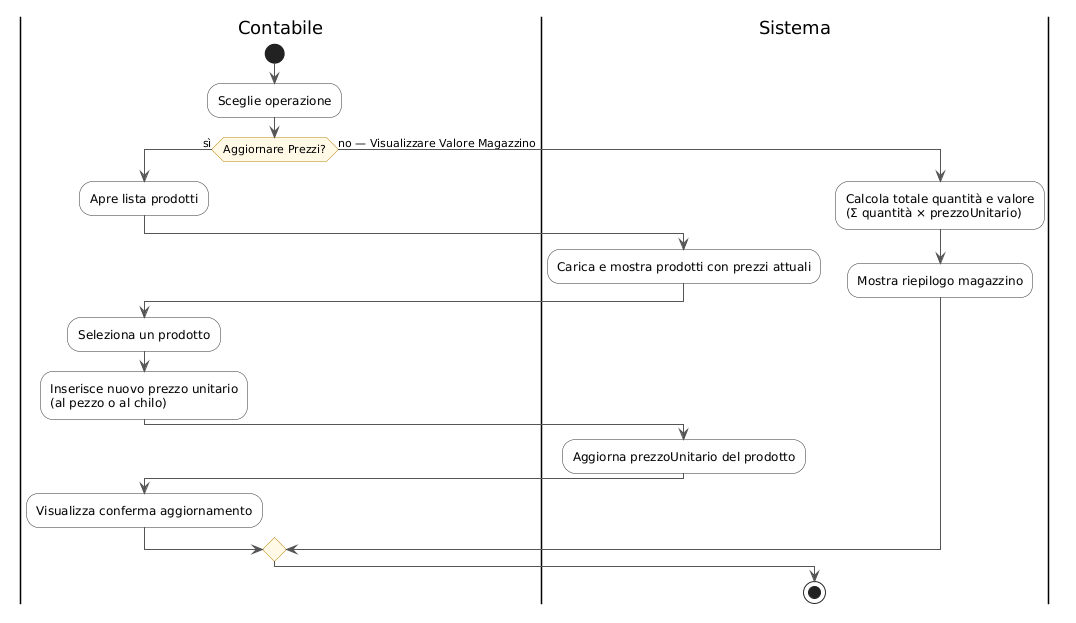
\includegraphics[width=0.8\textwidth]{./img/png-uml/UC7_ContabilePrezzi_AD.png}
    \caption{Diagramma di Attività: Contabile Prezzi (UC7)}
\end{figure}

\begin{figure}[h]
    \centering
    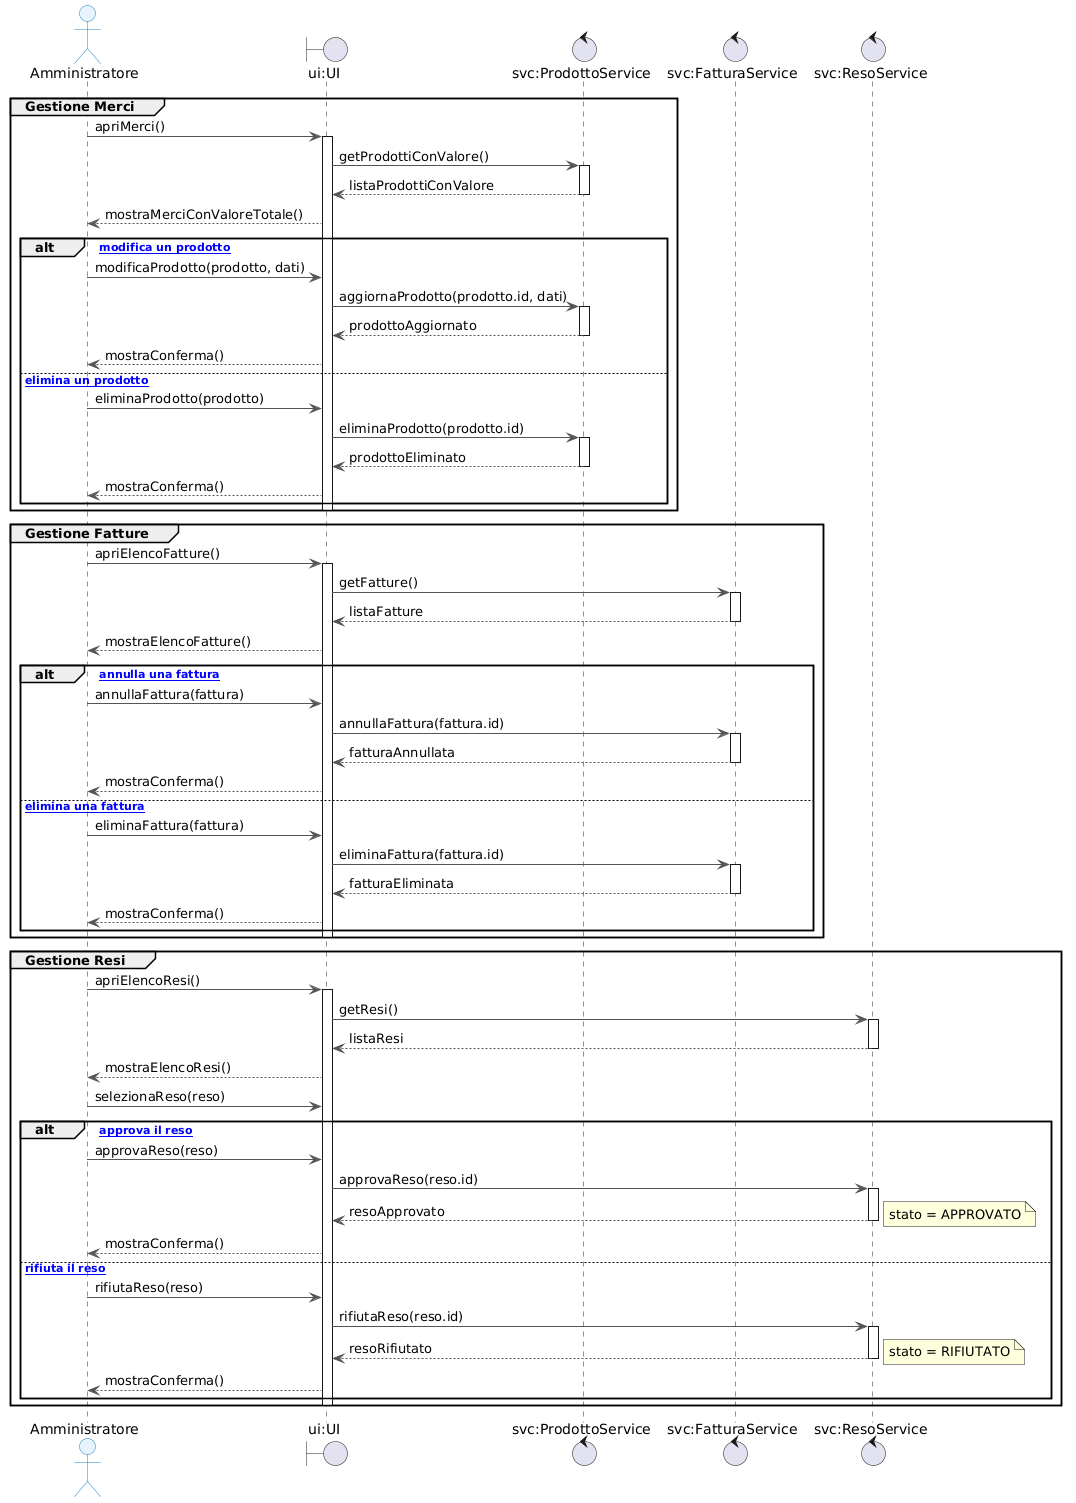
\includegraphics[width=0.8\textwidth]{./img/png-uml/UC8_Amministratore_SD.png}
    \caption{Diagramma di Sequenza: Amministratore (UC8)}
\end{figure}

\begin{figure}[h]
    \centering
    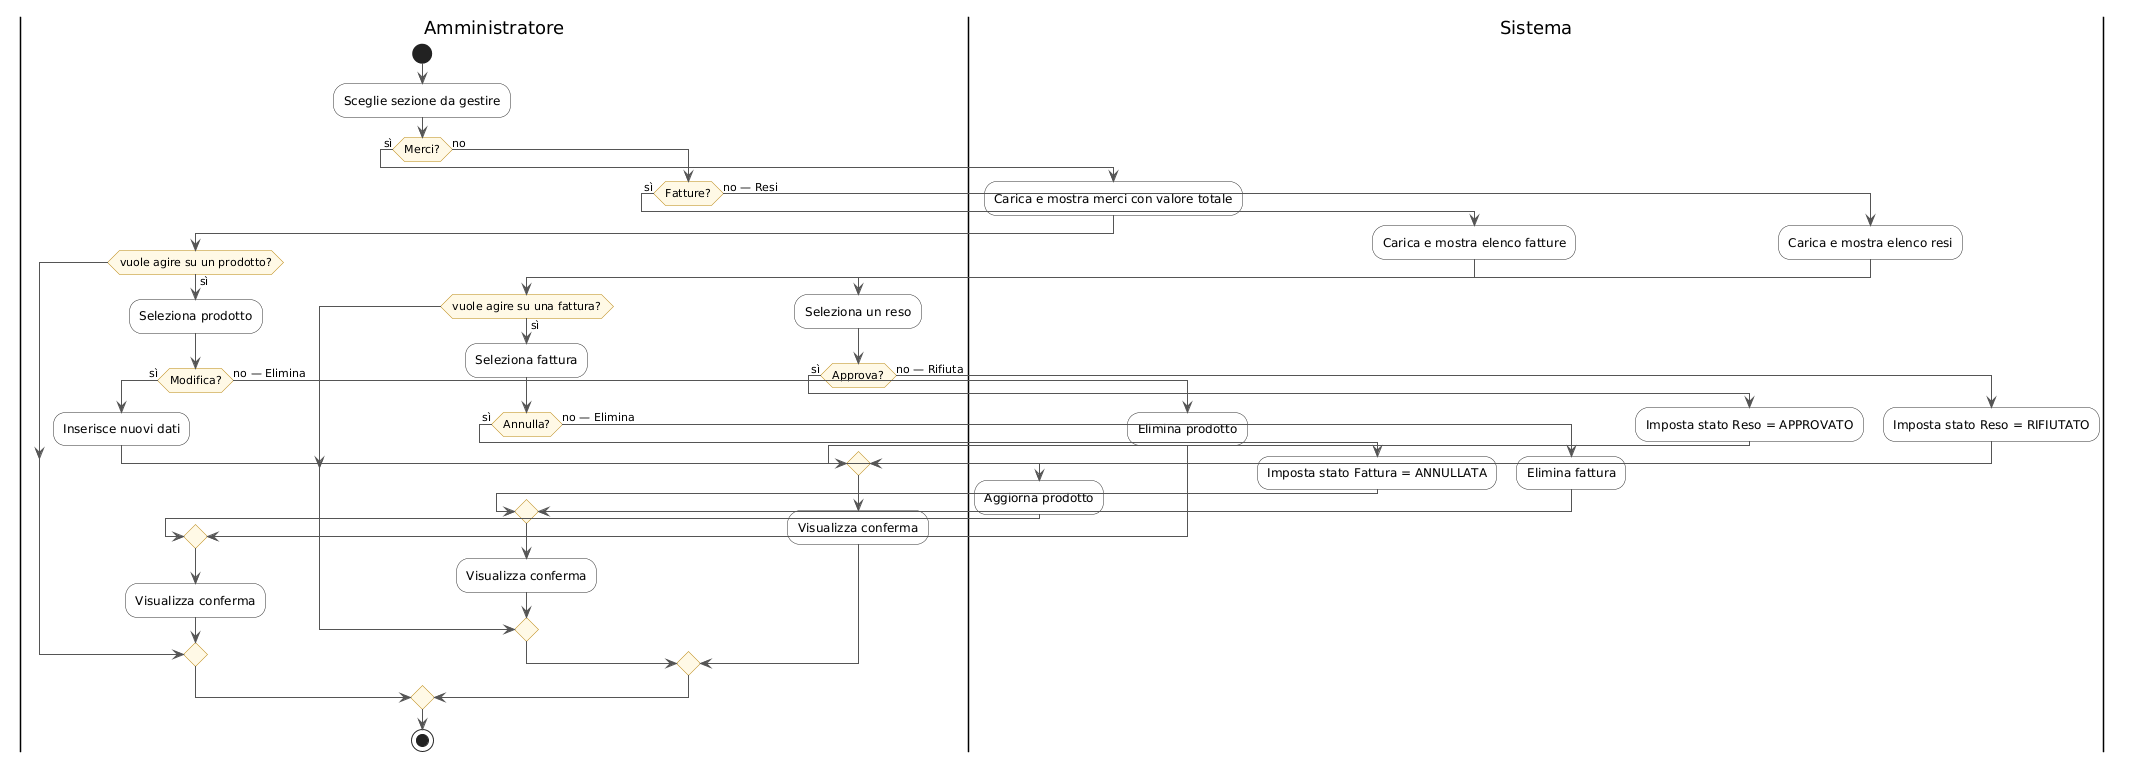
\includegraphics[width=0.8\textwidth]{./img/png-uml/UC8_Amministratore_AD.png}
    \caption{Diagramma di Attività: Amministratore (UC8)}
\end{figure}

\section{Gestione del Progetto (Scrum)}
\subsection{Backlog}
L'elenco ordinato e prioritizzato dei requisiti tecnici necessari al completamento del primo ciclo di sviluppo comprende:
\begin{enumerate}
    \item Configurazione dell'architettura software di base, dell'ambiente di sviluppo locale e della connessione al file SQLite.
    \item Definizione dello schema logico della base dati tramite script SQL (creazione delle tabelle \texttt{Utente}, \texttt{Prodotto}, \texttt{Categoria}, \texttt{Giacenza}, \texttt{OrdineEntrata}, \texttt{OrdineUscita}, \texttt{RigaOrdineEntrata}, \texttt{RigaOrdineUscita}, \texttt{DDT}).
    \item Sviluppo delle interfacce grafiche e delle funzioni CRUD per la gestione dell'Anagrafica Prodotti e Categorie.
    \item Implementazione del modulo di movimentazione (logica e maschere per la compilazione di \texttt{OrdineEntrata} e \texttt{OrdineUscita}).
    \item Integrazione software per l'acquisizione dell'input da lettore di codici a barre tramite emulazione tastiera.
    \item Sviluppo del sottosistema di controllo e notifica visiva per i prodotti sotto la soglia minima inseriti in \texttt{Giacenza}.
    \item Progettazione ed implementazione del motore di reportistica ed esportazione dell'inventario in formato PDF e CSV.
    \item Sviluppo del modulo di autenticazione locale e gestione dei permessi basata sui ruoli tramite \texttt{AuthService}.
\end{enumerate}

\subsection{User Stories}
Le storie riflettono i bisogni concreti degli attori scritti secondo gli standard del framework Scrum:
\begin{itemize}
    \item \textbf{US-01 (Accesso con credenziali)}: "Come utente, voglio accedere all'applicazione con username e password, in modo da poter utilizzare le funzionalità del mio ruolo".
    \item \textbf{US-02 (Scansione Barcode)}: "Come magazziniere, voglio poter scansionare il codice a barre di un prodotto in arrivo tramite il lettore ottico, per aggiornare la quantità in giacenza nel sistema in modo rapido, automatizzato e senza commettere errori manuali".
    \item \textbf{US-03 (Sicurezza Account)}: "Come amministratore del sistema, voglio che il software blocchi l'account dopo 3 tentativi falliti, per impedire ad utenti non autorizzati di indovinare le password d'accesso dei dipendenti".
    \item \textbf{US-04 (Recupero Password)}: "Come utente, voglio poter recuperare la mia password dimenticata rispondendo a una domanda di sicurezza preimpostata".
    \item \textbf{US-05 (Visualizzazione elenco ordini)}: "Come magazziniere, voglio vedere l'elenco di tutti gli ordini di entrata e uscita, in modo da avere una panoramica completa dei movimenti del magazzino".
    \item \textbf{US-06 (Visualizzazione dettaglio ordini)}: "Come magazziniere, voglio vedere il dettaglio di un ordine di entrata o uscita selezionato, in modo da conoscere i prodotti coinvolti e le relative quantità".
    \item \textbf{US-07 (Registrazione Ordini in entrata)}: "Come magazziniere, voglio registrare un ordine di entrata con i prodotti ricevuti, in modo da aggiornare automaticamente le giacenze".
    \item \textbf{US-08 (Registrazione Ordini in uscita)}: "Come magazziniere, voglio registrare un ordine di uscita con i prodotti richiesti, in modo da aggiornare automaticamente le giacenze".
    \item \textbf{US-09 (Generazione DDT)}: "Come magazziniere, voglio generare un documento di trasporto (DDT) per ogni ordine di uscita evaso, in modo da avere una documentazione ufficiale per la merce in uscita".
    \item \textbf{US-10 (Visualizzare Giacenze)}: "Come magazziniere, voglio visualizzare in tempo reale le giacenze di magazzino, in modo da sapere sempre la quantità disponibile di ogni prodotto".
    \item \textbf{US-11 (Stampa inventario)}: "Come magazziniere, voglio stampare un documento inventario, in modo da avere un registro fisico dello stato del magazzino".
    \item \textbf{US-12 (Gestione resi)}: "Come magazziniere, voglio gestire i resi della merce, in modo da poter ripristinare le quantità in giacenza e tenere traccia dei movimenti di reso".
    \item \textbf{US-13 (Visualizzazione ordini per contabile)}: "Come contabile, voglio visualizzare l'elenco degli ordini ricevuti (evasi e non evasi), in modo da poter gestire la fatturazione e le note di credito".
    \item \textbf{US-14 (Generazione Fatture)}: "Come contabile, voglio generare fatture per gli ordini di uscita evasi, in modo da poter emettere documenti ufficiali per i clienti".
    \item \textbf{US-14 (Gestione prezzi)}: "Come contabile, voglio poter modificare manualmente i listini dei prezzi di vendita e di acquisto dei prodotti, in modo da mantenere aggiornati i prezzi nel sistema".
    \item \textbf{US-15 (Reportistica inventario)}: "Come amministratore, voglio generare report avanzati dell'inventario, in modo da avere una visione dettagliata dello stato del magazzino e delle tendenze di consumo dei prodotti".
\end{itemize}

\subsection{Criteri di Accettazione}
Vengono definiti i vincoli formali affinché la User Story \textbf{US-01} possa essere considerata completata ("Done"):
\begin{itemize}
    \item \textbf{Criterio 1}: Il sistema deve riconoscere e decodificare correttamente e senza latenza i codici a barre conformi allo standard internazionale EAN-13.
    \item \textbf{Criterio 2}: Al momento della scansione riuscita all'interno della schermata di carico, i dati identificativi del prodotto devono comparire istantaneamente nei campi visivi e la relativa quantità nella tabella \texttt{Giacenza} deve essere incrementata automaticamente nel database.
    \item \textbf{Criterio 3}: Qualora il codice a barre scansionato non trovi corrispondenza all'interno della tabella \texttt{Prodotto}, il sistema deve inibire il salvataggio automatico, emettere un feedback acustico di errore ed aprire una finestra pop-up contestuale che consenta all'operatore di inserire il prodotto ex-novo in anagrafica o annullare l'operazione.
\end{itemize}

\section{Strategia di Verifica e Validazione}
\subsection{Piano di Testing}
Il piano prevede una suite di test di unità (Unit Testing) sistematici eseguiti sulla Business Logic tramite JUnit. I test sono focalizzati sulla verifica delle transazioni e sul rispetto dei vincoli di integrità del magazzino.

\subsection{Casi di Test (Test Cases)}
\textbf{TC-01}: Tentativo di scarico merce con quantità richiesta superiore alla giacenza fisica attuale.
\begin{itemize}
    \item \textbf{Scenario}: Un prodotto registrato in anagrafica dispone di una quantità fisica in \texttt{Giacenza} pari a 5 unità. Viene inserito un \texttt{OrdineUscita} con una \texttt{RigaOrdineUscita} richiedente l'uscita di 6 unità del medesimo prodotto.
    \item \textbf{Input}: Invocazione della funzione di business \texttt{registraScarico()} con quantità = 6.
    \item \textbf{Risultato Atteso}: Il sistema deve intercettare preventivamente l'incoerenza prima di modificare i dati, bloccare l'esecuzione della transazione sul database SQLite tramite un'operazione di \texttt{ROLLBACK} e sollevare un'eccezione software personalizzata di tipo \texttt{GiacenzaInsufficienteException}. L'interfaccia utente cattura l'eccezione e mostra un messaggio di errore bloccante, impedendo che i dati assumano valori negativi incongruenti.
\end{itemize}

\end{document}